%% MODELO DE LATEX PARA TRABALHOS ACADÊMICOS

\documentclass[
	% -- opções da classe memoir --
	12pt,				% tamanho da fonte
	% openright,			% capítulos começam em pág ímpar (insere página vazia caso preciso)
    oneside,			% para impressão somente frente. Oposto a twoside (frente e verso)
	a4paper,			% tamanho do papel. 
	% -- opções da classe abntex2 --
	%chapter=TITLE,		% títulos de capítulos convertidos em letras maiúsculas
	%section=TITLE,		% títulos de seções convertidos em letras maiúsculas
	%subsection=TITLE,	% títulos de subseções convertidos em letras maiúsculas
	%subsubsection=TITLE,% títulos de subsubseções convertidos em letras maiúsculas
	% -- opções do pacote babel --
	english,			% idioma adicional para hifenização
	french,				% idioma adicional para hifenização
	spanish,			% idioma adicional para hifenização
	brazil,				% o último idioma é o principal do documento
	]{abntex2}


% ---
% PACOTES
% ---

% ---
% Pacotes fundamentais 
% ---
\usepackage{cmap}				% Mapear caracteres especiais no PDF
\usepackage{lmodern}			% Usa a fonte Latin Modern
\usepackage[T1]{fontenc}		% Selecao de codigos de fonte.
\usepackage[utf8]{inputenc}		% Codificacao do documento (conversão automática dos acentos)
\usepackage{indentfirst}		% Indenta o primeiro parágrafo de cada seção.
\usepackage{color}				% Controle das cores
\usepackage{graphicx}			% Inclusão de gráficos
\usepackage{epigraph}
\usepackage{multicol}
\usepackage{multirow}
\usepackage{lipsum}				% para geração de dummy text
\usepackage[brazilian,hyperpageref]{backref}	 % Paginas com as citações na bibl
\usepackage[alf]{abntex2cite}	% Citações padrão ABNT



% --- 
% CONFIGURAÇÕES DE PACOTES
% --- 

% ---
% Configurações do pacote backref
% Usado sem a opção hyperpageref de backref
\renewcommand{\backrefpagesname}{Citado na(s) página(s):~}
% Texto padrão antes do número das páginas
\renewcommand{\backref}{}
% Define os textos da citação
\renewcommand*{\backrefalt}[4]{
	\ifcase #1 %
		Nenhuma citação no texto.%
	\or
		Citado na página #2.%
	\else
		Citado #1 vezes nas páginas #2.%
	\fi}%
% ---

% ---
% Informações de dados para CAPA e FOLHA DE ROSTO
% ---
\titulo{SysNut - Um sistema de auxílio ao Nutricionista}
\autor{Linneu Magno Lopes de Sousa  
	   \\ Orientadora: Professora Ma. Patricia Medyna Lauritzen
de Lucena Drumond
   	   \\ Co-orientador: Jonnison Lima Ferreira %Caso Haja
	   }
\local{Picos - PI}
\data{10 de novembro de 2017}
\instituicao{%
  Universidade Federal do Piauí
  \par
  Campus Senador Heuvídio Nunes de Barros 
  \par
  Bacharelado em Sistemas de Informação}
\tipotrabalho{Monografia}
% O preambulo deve conter o tipo do trabalho, o objetivo, 
% o nome da instituição e a área de concentração 
\preambulo{Trabalho de Conclusão de Curso apresentado ao
Curso de Bacharel em Sistemas de Informação,
Campus Senador Helvídio Nunes de Barros, da
Universidade Federal do Piauí como parte dos
requisitos para obtenção do referido grau.}
% ---

% ---
% Configurações de aparência do PDF final

% alterando o aspecto da cor azul
\definecolor{blue}{RGB}{41,5,195}

% informações do PDF
\makeatletter
\hypersetup{
     	%pagebackref=true,
		pdftitle={\@title}, 
		pdfauthor={\@author},
    	pdfsubject={\imprimirpreambulo},
	    pdfcreator={LaTeX with abnTeX2},
		pdfkeywords={abnt}{latex}{abntex}{abntex2}{relatório técnico}, 
		colorlinks=true,       		% false: boxed links; true: colored links
    	linkcolor=blue,          	% color of internal links
    	citecolor=blue,        		% color of links to bibliography
    	filecolor=magenta,      		% color of file links
		urlcolor=blue,
		bookmarksdepth=4
}
\makeatother
% --- 


% ---
% compila o indice
% ---
\makeindex
% ---







% ----
% Início do documento
% ----
\begin{document}

% Retira espaço extra obsoleto entre as frases.
\frenchspacing 

% ----------------------------------------------------------
% ELEMENTOS PRÉ-TEXTUAIS
% ----------------------------------------------------------
% \pretextual

% ---
% Capa
% ---
\imprimircapa
% ---

% ---
% Folha de rosto
% (o * indica que haverá a ficha bibliográfica)
% ---
\imprimirfolhaderosto*
% ---






% ---
% Agradecimentos
% ---
\begin{agradecimentos}

	Pai Celestial, sou grato eternamente por tua bondade e misericórdia. O Senhor me manteve confiante em busca dos meus sonhos.

	A minha família, agradeço por toda a confiança, apoio e incentivo. Meus pais: Milton José de Sousa e Maria Luzanilda Lopes de Carvalho Sousa, meus irmãos: Ludmilla Moema Lopes de Sousa e Lamarck Mendel Lopes de Sousa. Tenho certeza de que essa conquista não seria possível sem vocês, pois desde o início, foi em quem me espelhei e busquei forças para continuar. Foi também por vocês que busquei essa conquista e que buscarei ainda mais.

	Sou muito grato a minha namorada: Mayara Teresa de Carvalho. Pelo amor, pelo carinho, pelo apoio, inclusive profissional. Você também tornou esse sonho possível. Muito obrigado, meu amor.

	Aos meus mestres, desde o meu primeiro ano na escola até o último período de faculdade. Se existe um profissional que merece ser reconhecido pelo seu trabalho e sua função na sociedade, este precisa ser o professor. Muito obrigado pelo conhecimento compartilhado. Agradeço em especial aos meus orientadores: Ismael de Holanda Leal e Patricia Medyna Lauritzen de Lucena Drumond e meu coorientador Jonnison Lima Ferreira, por dedicarem parte do seu tempo para aperfeiçoar meu trabalho e também tornar essa conquista possível.

	Aos meus amigos, irmãos DeMolay’s e tios maçons. Durante todos esses anos enquanto estive aqui para obter o grau de bacharel em Sistemas de Informação, vocês também fizeram parte do alicerce que me sustentou.

	Eu realmente agradeço a todos que contribuíram direta ou indiretamente para essa conquista. Muito obrigado a todos!


\end{agradecimentos}
% ---

% ---
% Epigrafe
% ---
\vspace*{\fill}
{ \raggedleft
	\textit{Não a nós, Senhor, nenhuma glória para nós, mas sim ao teu nome, por teu amor e por tua fidelidade!. \\
		Salmos 115:1}
	~
}
\pagebreak


% ---
% RESUMO
% ---

% resumo na língua vernácula (obrigatório)
\begin{resumo} %% AQUI COMEÇA A PÁGINA DE RESUMO
 A alimentação é muito importante na vida humana. Devido a vida corriqueira das
pessoas, aumentou-se a demanda pelos \textit{fast-food}, alimentos estes ricos em
substâncias prejudiciais à saúde, causadores das doenças crônicas não transmissíveis. 
A preocupação com a melhora e qualidade de vida faz com que as pessoas busquem cada
vez mais o nutricionista. Por outro lado, o
nutricionista encontra um trabalho que necessita de organização e precisão, do
contrário pode cometer erros que comprometam o seu trabalho com o paciente. Diante
dessas dificuldades, surge a demanda por ferramentas que auxiliem o trabalho do
nutricionista, possibilitando um trabalho com mais agilidade e atenção às
necessidades do seu cotidiano profissional. O sistema deste trabalho propõe uma
ferramenta simples, ao tempo que proporciona uma boa
experiência para o profissional que a utiliza e consequentemente reduz o índice de
obesidade iminente.
 \vspace{\onelineskip}
    
 \noindent
 \textbf{Palavras-chaves}: Alimentação, Sistema de apoio ao
nutricionista, obesidade.
\end{resumo} %AQUI TERMINA A PÁGINA DE RESUMO


\begin{resumo}[Abstract]
Food is very important in human life. Because of people's everyday lives, the demand for fast food has increased. This kind of food is rich in substances harmful to health, chronic non-communicable diseases. The concern with the improvement and quality of life causes people to seek more and more the nutritionist. On the other hand, the nutritionist finds a job that needs organization and accuracy. Inconsequence, he may make mistakes that compromise his work with the patient. Faced with these difficulties, there is a demand for tools that help the nutritionist's job. This work proposal consists on a simple tool and providing a good experience for the professional who uses it and consequently reduces the rate of imminent obesity.
\vspace{\onelineskip}

\noindent
\textbf{Keywords}: Food, Nutritionist support system, obesity.
\end{resumo}


% ---
% inserir lista de ilustrações
% ---

\listoffigures* %% o * indica que não será incluso no sumário
\cleardoublepage %% Pula página
% ---

% ---
% inserir lista de tabelas
% ---

%\listoftables*
%\cleardoublepage
% ---

% ---
% inserir lista de abreviaturas e siglas
% ---

\begin{siglas}
	\item[DCNT] Doenças Crônicas Não Transmissíveis
 	\item[CSS] \textit{Cascading Style Sheets}
	\item[DRY] \textit{Don’t Repeat yourself}
	\item[ETA] Efeito Térmico dos Alimentos
	\item[GPL] \textit{General Public License}
	\item[HTML] \textit{HyperText Markup Language}
	\item[ITIL] \textit{Information Technology Infrastructure Library}
	\item[JSON] \textit{JavaScript Object Notation}
	\item[MVC] \textit{Model-View-Controller}
	\item[MTV] \textit{Model-Template-View}
	\item[NSF] \textit{National Science Foundation}
	\item[OMG] \textit{Object Management Group}
	\item[ORM] \textit{Object-relational mapper}
	\item[PSF] \textit{Python Software Foundation}
	\item[SGBD] Sistema de Gerenciamento de Banco de Dados
	\item[SP] \textit{Story points}
	\item[SQL] \textit{Structured Query Language}
	\item[TACO] Tabela Brasileira de Composição de Alimentos
	\item[TMB] Taxa Metabólica Basal
	\item[GET] Gasto Energético Total
	\item[URL] \textit{Uniform Resource Locator}
	\item[UML] \textit{Unified Modeling Language}
	\item[VBA] \textit{Visual Basic for Applications}
	\item[VN] Valor de negócio
	\item[XML] \textit{Extensible Markup Language}
\end{siglas}
% ---

% ---
% inserir lista de símbolos
% ---
%\begin{simbolos}
%  \item[$ \Gamma $] Letra grega Gama
%  \item[$ \Lambda $] Lambda
%  \item[$ \zeta $] Letra grega minúscula zeta
%  \item[$ \in $] Pertence
%\end{simbolos}
% ---

% ---
% inserir o sumario
% ---

\tableofcontents*

% ---

% ----------------------------------------------------------
% ELEMENTOS TEXTUAIS  (necessário para incluir número nas páginas)
% ----------------------------------------------------------
\textual


% ----------------------------------------------------------
% Introdução
% ----------------------------------------------------------
\chapter{Introdução} %% NOVO CAPÍTULO (REPARE QUE ELE AUTOMATICAMENTE JÁ COLOCA O NÚMERO DO CAPÍTULO E JÁ ADICIONA NO SUMÁRIO)



A alimentação é um dos momentos mais importantes na vida das pessoas tanto
por fatores quanto por fatores sociais, culturais e científicos. É
por meio dela que se obtém a energia necessária para desenvolver atividades diárias
e outros nutrientes primordiais a saúde, como vitaminas e minerais. \cite{proenca}.

O Brasil atualmente passa por uma etapa de transição na alimentação de sua
população, a mesma que antes enfrentava a desnutrição, nos dias atuais apresenta
alta prevalência de obesos, isso pode ser explicado pela mudança drástica na
alimentação. Com o aumento da renda básica das famílias, o \textit{fast-food} tornou-se
presente nas mesas da população brasileira. Alimentos como estes, são ricos em
gordura saturada, açúcar e sódio, os quais são precursores de diversas doenças crônicas não
transmissíveis (DCNT) como, diabetes mellitus tipo II, doenças no sistema
cardiovascular, obesidade mórbida, entre outras \cite{schuster}.
A preocupação com a alimentação e qualidade de vida se faz cada
dia mais presente no cotidiano de todos os brasileiros, decorrência do uso exacerbado
dos \textit{fast-food}. O nutricionista, 
profissional responsável pela prescrição dietoterápica, tem ganho mais cada vez mais espaço no mercado de
trabalho, perante sua importância para manutenção da saúde do ser humano
\cite{brasil}.

Diante da importância do seu trabalho, o nutricionista tem buscado melhorias
no seu atendimento, que por vezes torna-se cansativo perante a vasta quantidade de
cálculos para análise do estado nutricional do paciente, das necessidades energéticas
e para adequação do cardápio. A necessidade de agilizar e aprimorar o atendimento
nutricional acarretou o surgimento de softwares que atendessem as necessidades
básicas como resolução de equações e maior organização dos dados dos pacientes
\cite{vieira}.

A ferramenta proposta neste trabalho, além de ajudar o nutricionista em seu cotidiano de trabalho,
também contribui com a redução do índice de obesidade existente no Brasil, através da utilização da mesma
de forma totalmente gratuita por parte de profissionais da nutrição que acabaram de ingressar no mercado
de trabalho e ainda não possuem nenhuma ferramenta que auxiliem a sua rotina.


\section{Contexto e Problema}

Durante o acompanhamento do paciente, o nutricionista muitas vezes precisa
consultar diversos autores para efetuar um trabalho com mais precisão. Esta etapa do trabalho do profissional
torna-se bastante dificultoso sem o auxílio de uma ferramenta que faça a pesquisa e efetue os cálculos automaticamente.

Para \citeonline{araujo}, antropometria ou avaliação antropométrica é um importante método para avaliação do estado nutricional de um indivíduo e possibilita a detecção de alteração do estado nutricional do mesmo ou até mesmo de coletividades. A Organização Mundial da Saúde (OMS) afirmou em 1995 que a avaliação antropométrica é uma importante ferramenta para detecção para grupos, mas que não deve ser utilizada para diagnóstico final \cite{oms}.

O acompanhamento nutricional individualizado é extremamente importante para
o paciente obter resultados relevantes de acordo com o objetivo traçado pelo
nutricionista, visto que, cada indivíduo possui uma necessidade energética diferente
e a distribuição dos macronutrientes e micronutrientes é realizada de acordo com seu
tipo de organismo, objetivo a ser alcançado e estado nutricional, mediante avaliação
antropométrica.
O nutricionista necessita usar diversas fórmulas
e equações no seu dia a dia, seja para avaliar o estado nutricional do
paciente ou para esquematizar um plano alimentar, fórmulas essas que nem sempre
são sinônimos de praticidade e simplicidade. Esse fator pode trazer perdas
significativas ao profissional da nutrição, visto que são necessários vários cálculos
para prestar atendimento adequado ao seu público-alvo.

Diante disso, é imprescindível uma ferramenta computacional que possibilite a inclusão de refeições, troca de mensagens entre
os usuários do sistema (paciente e nutricionista), 
cálculo das necessidades energéticas e analise do
cardápio auxiliando o profissional durante seu atendimento, trazendo mais
comodidade e rapidez ao seu serviço prestado, de qualquer dispositivo que esteja acessando, desde
que tenha acesso à internet.

\section{Objetivos}

Esse trabalho teve como objeto o desenvolvimento de um sistema para
nutricionistas, voltado para o atendimento nutricional de seus pacientes, atendendo
todas as necessidades primárias de um atendimento individualizado.

\section{Organização do trabalho}
Este trabalho está organizado da seguinte maneira:

 \begin{itemize}

	\item Capítulo 2 - Descreve descritas todas as ferramentas e técnicas que foram utilizadas durante o desenvolvimento do sistema.
	\item Capítulo 3 – Discute alguns dos trabalhos encontrados que possuem relação com o trabalho do autor.
	\item Capítulo 4 – Explica como o sistema foi implementado e relaciona os casos de uso.
	\item Capítulo 5 – Apresenta e discute os resultados da implementação do projeto.
	\item Capítulo 6 - Aborda os principais achados previstos pelo autor.

\end{itemize}

% ---
% Capitulo de revisão de literatura
% ---
\chapter{Referencial Teórico}

Este capítulo é destinado a discussão dos conceitos utilizados durante o desenvolvimento do projeto. \citeonline{tenorio} ressalta a importância da organização e compreensão das informações de um sistema \textit{web} por parte do usuário, atendendo às necessidades e exigências do mesmo durante o desenvolvimento do sistema.

% --- Seção dentro do capítulo
\section{Servidor}
% ---

O lado servidor é onde deve funcionar a lógica principal da aplicação. Todas as
ações são tratadas como requisição. Quando o usuário faz a requisição ao servidor,
é chamado de HTTP \textit{request}. Quando a resposta é enviada pelo servidor, esta ação
é chamada de HTTP \textit{response}.

Os sistemas \textit{web} funcionam da seguinte maneira: o usuário (cliente) faz uma
requisição de uma página para o servidor e retorna uma resposta para ele através do
navegador. A resposta é interpretada pelo navegador e entregue pelo servidor para o
usuário \cite{niederauer}.

\subsection{Python}

Python é uma linguagem de programação de altíssimo nível, orientada a objeto
e de tipagem dinâmica e forte, interpretada e interativa. O nome Python foi dado por
Guido van Rossum do programa da TV Britânica \textit{Monty Python’s Flying Circus} e a
linguagem foi criada por ele, na década de 90, no Instituto Nacional de Pesquisa para
Matemática e Ciência da Computação da Holanda (CWI). O Python foi concebido a
partir de outra linguagem existente na época, chamada ABC.

A intenção do autor ao criar a linguagem é que fosse de altíssimo nível e que
tivesse características importantes de outras linguagens de programação. Python é
livre, ou seja, tem código aberto, com licença compatível com a \textit{General Public License}
(GPL). A especificação da linguagem é mantida pela \textit{\textit{Python Software Foundation}}
(PSF). A linguagem Python apresenta uma série de vantagens e recursos
interessantes que foram inspirados e aproveitados de outras linguagens de sucesso,
tornando-a assim uma linguagem bastante flexível \cite{borges}.

Python possui diversas características e estruturas de alto nível (listas,
dicionários, entre outros) e uma coleção de módulos prontos para uso, além de outras
ferramentas que podem ser utilizadas para auxiliar no desenvolvimento, dentre elas
citamos o Django, que será abordado no tópico a seguir.

Segundo \citeonline{diakopoulos}, Python lidera o ranking de linguagens
mais utilizadas, seguido por C e Java. Existem também implementações de Python
para .NET (IronPython), JVM (Jython), entre outros.

\subsection{Django}

O Django é um \textit{framework} de desenvolvimento \textit{web} criado por Jacob KaplalnMoss,
Adrian Holovaty e Simon Willison em 2003. O Django utiliza o conceito DRY –
\textit{Don’t Repeat yourself} (“não repita a si mesmo”), que propõe que cada parte de um
sistema deve possuir uma representação única.

O Django possui vários componentes com funções específicas. \citeonline{neto}
cita alguns de seus principais componentes:

 \begin{itemize}

	\item \textbf{ORM} \textit{\textit{Object-relational mapper}} (Mapeador objeto-relacional): é
uma técnica de mapeamento objeto relacional que permite fazer uma
relação dos objetos com os dados que estes representam.
	\item \textbf{\textit{Template System}}: linguagem para criação de templates (HTML, XML,
JSON, etc.) usados na geração de páginas dinâmicas.
Sistema de administração: Interface de administração própria do
\textit{framework} (Django-admin).
	\item \textbf{URL} (\textit{Uniform Resource Locator}) \textit{dispatcher}: Processador de URLs
do sistema que executando funções específicas feitas pelo
desenvolvedor, possibilitando URL’s amigáveis.
	\item \textbf{Internacionalização}: Permite que o sistema seja traduzido para
diversos idiomas.
	\item \textbf{Formulários}: geração automática de formulários e facilitação na
manipulação dos dados enviados por meio deles.
	\item \textbf{Segurança}: gerenciamento de autenticação de usuários e controle de
permissões.
	\item \textbf{Outros componentes}: serialização de dados, sistema de testes
automatizado, entre outros.

\end{itemize}

O Django utiliza o padrão de projeto MTV (\textit{Model-Template-View}) para
desenvolvimento, que possui essencialmente a mesma lógica que o MVC (\textit{Model-View-Controller}),
muito utilizado em outras linguagens \cite{neto}.

O padrão de projeto MVC divide-se em três camadas: Modelo, Visão e
Controlador. O Modelo é o responsável pela comunicação com os dados
armazenados no banco de dados que serão visualizados na camada de Visão. A
Visão, por sua vez, é responsável pela apresentação da aplicação. E por último, o
controlador, responsável por administrar todo o fluxo da aplicação \cite{lemos}.


\subsection{Banco de Dados MySQL}
O MySQL, criado pela empresa MySQL AB na Suécia, é um SGBD que utiliza a
linguagem SQL como interface. A MySQL AB foi adquirida pela Sun Microsystems em
2008, a qual posteriormente foi comprada pela Oracle, incluindo o SGBD MySQL.

Atualmente, esse é um dos bancos de dados mais utilizados do mundo, com mais de
10 milhões de instalações e um dos motivos para essa popularidade é devido a fácil
integração a também popular linguagem PHP \cite{mottin}.

O MySQL é o banco de dados de código aberto mais popular do mundo. Ainda
mantido pela Oracle, tornou-se a principal escolha de banco de dados para aplicativos
\textit{web}, usado por \textit{websites} muito conhecidos como: Facebook, Twitter, YouTube, entre
outros.

% --- Seção dentro do capítulo
\section{Cliente}
% ---

O lado cliente de uma aplicação \textit{web} é quem realiza a requisição e se comunica
com o servidor, ao tempo que recebe a resposta do mesmo. Em outras palavras, o
lado cliente é quem estabelece a comunicação com o usuário.

\subsection{HTML}

HTML é uma sigla em inglês que significa Linguagem para Marcação de
Hipertexto (\textit{HyperText Markup Language}). Na aplicação, é usada para denotar os 
elementos da página, tais como caixas de seleção, caixas de texto, etc. Sua função é
definir apenas a estrutura da página \cite{folle}.A Figura 1 é um exemplo simples de uma página com código HTML, mostrando
algumas tags HTML e suas funcionalidades de marcação:

\begin{figure} [hbt] 
%% hbt SIGNIFICA QUE ELE PRIMEIRO VAI TENTAR COLOCAR A IMAGEM NESTE LUGAR (h de "here"). SENÃO DER, ELE TENTA COLOCAR MAIS PRA BAIXO (b de "bottom"). SENÃO ELE COLOCA MAIS PARA CIMA (t de "top").
\label{figura1} 
%% LABEL SERVE PARA VOCÊ REFERENCIAR A FIGURA NO MEIO DO TEXTO (VEJA LINHA 330: \ref{figura1}). ASSIM VOCÊ NÃO PERDE A REFERÊNCIA QUANDO MUDA A FIGURA DE LUGAR
\caption{Exemplo de código HTML.}
\begin{center}
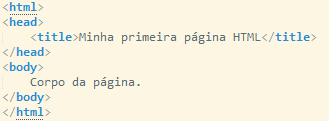
\includegraphics[width=0.75\textwidth]{exhtml.png} %% PARA COLOCAR O ARQUIVO DA IMAGEM NO SHARELATEX, CLIQUE NO ÍCONE QUE PARECE UMA FLECHINHA PARA CIMA (ATUALIZAR), CLIQUE EM UPLOAD E PROCURE A IMAGEM EM SEU COMPUTADOR.
\end{center}
\end{figure}

\begin{itemize}

	\item Tag <html> - delimita o início e o fim de uma página HTML. Tudo que
	\item Tag <head> - contém informações de cabeçalho da página, como: título,
	\item Tag <title> - Define o título da página.
	\item Tag <body> - Delimita o conteúdo que estará no corpo da página.

\end{itemize}


\subsection{\textit{Cascading Style Sheets} – CSS}

CSS (\textit{Cascading Style Sheets}) – é uma linguagem utilizada para tratamento
visual dos elementos da página \textit{web} \cite{folle}. Este é, portanto, a tecnologia
responsável por tratar cada elemento da página \textit{web} visualmente, atribuindo cores e
posições diferentes, dependendo da preferência do programador. Possui sintaxe
simples e assim como as demais tecnologias, utiliza-se de várias palavras em inglês
para especificar os diferentes estilos de propriedades da página.

\begin{figure} [hbt] 
\label{figura1} 
\caption{Exemplo de código CSS.}
\begin{center}
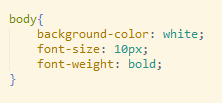
\includegraphics[width=0.75\textwidth]{excss.png}
\end{center}
\end{figure}

\subsection{\textit{JavaScript e JQuery}}

Segundo \citeonline{folle}, \textit{JavaScript} “é uma linguagem de script executada pelos
navegadores que permite o acesso e manipulação programática de objetos de uma
página \textit{web}”. Ela possibilita que um campo para digitar uma data seja formatado
automaticamente (com barras), ou que um campo seja desabilitado dinamicamente,
etc. 

\textit{Jquery} é portanto, uma biblioteca de funções prontas de \textit{JavaScript}, que
interagem com o HTML e possibilitam uma melhor experiência ao usuário. Foi lançada
em 2006, no BarCamp, de Nova York, por John Resig e é utilizada por milhares de
sites visitados pelo mundo. Segundo a \citeonline{w3techs}, é a biblioteca JavaScript
mais popular dentre as existentes

% --- Seção dentro do capítulo
\section{Engenharia de Software}
% ---
Segundo \citeonline{rohden}, “a Engenharia de Software propõe métodos
sistemáticos com o uso adequado de ferramentas e técnicas, que levam em
consideração o problema a ser resolvido, necessidades dos clientes e os recursos
disponíveis”. Considerando estes elementos, para obter software de qualidade, esta
engenharia é imprescindível, pois leva em consideração os principais elementos a
serem estudados e avaliados.


\subsection{\textit{Scrum}}
\textit{Scrum} é uma metodologia de desenvolvimento ágil que prioriza explicitamente
o retorno de investimento. O \textit{Product Owner} (pessoa que define os itens importantes
que compõe o \textit{Product Backlog}) tem a função de maximizar e priorizar as atualizações
do \textit{Product Backlog}, que é a lista de funcionalidades desejadas no desenvolvimento
do produto, de forma que os itens de maior valor para o cliente em cada momento
sejam implementados primeiro. Dessa forma, o incremento ao produto realizado ao
final de cada \textit{sprint} (itens desenvolvidos em um ciclo) gera retorno ao cliente por
diversas vezes ao longo do projeto \cite{machado}. 

\citeonline{machado} enfatizam ainda que saber responder as mudanças é mais
importante do que seguir um plano. Por se tratar de um \textit{framework} ágil, \textit{Scrum} encara 
as mudanças como parte natural do processo de desenvolvimento, através das
atualizações do \textit{Product Backlog}, onde as novas solicitações do cliente podem ser
introduzidas no próximo \textit{sprint}, gerando vantagem competitiva para as empresas.

\begin{figure} [hbt] 
\label{figura1} 
\caption{Ciclo de Desenvolvimento Scrum \cite{vascharim}}
\begin{center}
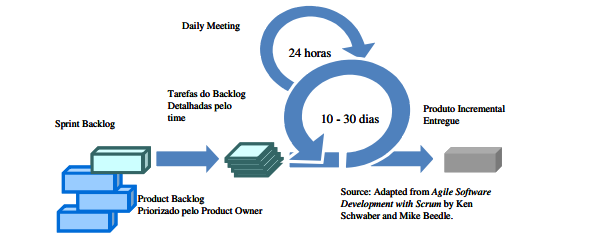
\includegraphics[width=0.75\textwidth]{scrum.png}
\end{center}
\end{figure}

A Figura 3 apresenta o ciclo de desenvolvimento \textit{Scrum}, que é dividido em
\textit{Sprints}, que podem durar de 10 a 30 dias e no final do \textit{sprint} é mostrado ao \textit{Product
Owner}. Durante cada \textit{sprint} são realizadas verificações do andamento do projeto. Um
conjunto de \textit{sprints} que formam uma versão utilizada do produto é chamado de
\textit{release}.

\subsection{Linguagem de Modelagem Unificada (\textit{Unified Modeling Language} – UML)}

Segundo \citeonline{costa}, a UML surgiu da união de métodos anteriores para
análise e projeto de sistemas orientados a objetos e em 1997 passou a ser aceita e
reconhecida como um padrão potencial de notação para modelagem de múltiplas
perspectivas de sistemas de informações pela OMG (\textit{Object Managment Group}). 

A UML oferece um suporte direto para o projeto e
implementação de cada perspectiva do sistema em desenvolvimento e também uma
notação para sua representação. Neste sistema, a UML foi importante durante todo o
processo sobretudo para visualização das funcionalidades e sua posterior 
implementação, bem como novas solicitações feitas pelo cliente. A UML apresenta
atores e onde podem estar representados suas ações no sistema, facilitando a
visualização do papel destes no sistema.

\section{Taxa Metabólica Basal (TMB)}

A taxa metabólica basal (TMB) é a quantidade de energia necessária para a
conservação das funções vitais do organismo, representando a maior parte do
consumo energético diário em humanos (cerca de 50\% a 70\%). Sendo calculada em
condições padrão de jejum, repouso físico e mental em ambiente calmo com controle
de temperatura, iluminação e barulhos \cite{ruiz} \cite{harris1}.

A TMB sofre grande influência da massa magra, sexo, idade, composição
corporal e predisposição genética. Fatores como o funcionamento do sistema nervoso
e os hormônios tireoidianos, também contribuem para diferença da TMB entre os
indivíduos. Para a estimativa da TMB, foram desenvolvidas várias equações
matemáticas, utilizando variáveis de fácil mensuração e de baixo custo, como idade,
altura e massa corporal total. Entre tantas equações, são utilizadas as seguintes:
\citeonline{harris1}, sua reformulação \citeonline{harris2} e \citeonline{cunningham} por possuírem grande
aceitabilidade e credibilidade pelas entidades relacionadas a Nutrição \cite{weijs}.

Esse cálculo torna-se indispensável durante o atendimento nutricional, visto
que ele é responsável pela individualização da sua dieta, de forma que possa atender
todas as necessidades calóricas do mesmo, auxiliando na melhora do quadro
nutricional do paciente \cite{pedrosa}.

O sistema deve então focar nos dados que estas fórmulas podem apresentar
como resultado, a fim de que possa facilitar o atendimento por parte do nutricionista,
ao tempo que o paciente obtenha um resultado com maior satisfação.


\section{Gasto Enérgico Total (GET)}

O gasto energético total (GET) compreende a soma de todos os gastos energéticos diários a seguir: A
taxa metabólica basal (TMB) que compreende o gasto energético necessário para a
consumação das funções vitais do organismo; o gasto energético da atividade física
ou fator de atividade (FA), que representa o gasto calórico com as atividades físicas
do cotidiano e o exercício físico; e o efeito térmico dos alimentos (ETA), relacionado
com a digestão, a absorção e o metabolismo dos alimentos. Em indivíduos saudáveis,
a TMB corresponde aproximadamente de 60\% a 70\% do gasto diário, o ETA entre 5\% 
e 15\% e o GEAF ou FA de 15\% a 30\%, sendo este último o elemento que mais varia
entre os indivíduos \cite{hill}. 

\section{TACO - Tabela Brasileira de Composição de Alimentos}

Reconhecida oficialmente pelo Ministério da Saúde e produzida pela Universidade de Campinas, o objetivo da TACO é gerar dados sobre a composição dos principais alimentos consumidos no Brasil, de maneira que possa assegurar a confiabilidade dos resultados \cite{taco}. 

Para desenvolver o sistema, foi necessário utilizar-se de um banco de dados que dispusesse das informações nutricionais necessárias para fazer a anamnese alimentar. Para isto, esta ferramenta foi escolhida. A tabela possui mais de 1000 alimentos cadastrados e informa detalhadamente a composição de cada alimento.

\section{\textit{Bootstrap}}

\textit{Bootstrap} é o mais popular \textit{framework} de HTML, CSS e \textit{JavaScript} para desenvolvimento de sistemas \textit{web} de modo responsivo. Esta ferramenta conta com centenas de classes que auxiliam na construção de uma página \textit{web} \cite{bootstrap}.

Esta ferramenta está presente em cada página do sistema, possibilitando que ele seja acessado de qualquer dispositivo (móvel ou \textit{desktop}). A sua versão estável é a 3.3.7, mas já foi disponibilizada oficialmente a versão 4, versão esta utilizada neste projeto.
\chapter{Trabalhos Relacionados}

Este capítulo apresenta uma relação de trabalhos com temas relacionados a este. Durante a pesquisa, pode-se concluir que ainda não é muito comum encontrar trabalhos científicos que envolvam desenvolvimento de sistema \textit{web}. 

\section{Desenvolvimento de um \textit{software} para avaliação nutricional antropométrica utilizando \textit{Visual Basic for Applications}}

O trabalho de \citeonline{alves} é voltado para \textit{desktop} e possui área em comum em relação a este trabalho. O autor utiliza o VBA, uma implementação feita pela Microsoft para os seus programas. O autor faz um comparativos com alguns produtos de mesmo tema que encontrou no mercado no ano da publicação.

O referido trabalho possui poucas ferramentas em comuns, inclusive por ter aplicação diferente. O sistema que o autor desenvolveu possui pouca portabilidade e compatibilidade, mas se apresenta como um sistema simples e prático. Também utiliza-se do mesmo banco de dados que este trabalho utilizou para cadastrar alimentos com suas informações nutricionais: a tabela TACO.


\section{Desenvolvimento e implantação de um sistema de chamadas com foco no ITIL, utilizando-se \textit{Python}, \textit{Django}, \textit{Highcharts} e \textit{Twitter Bootstrap}}

Neste trabalho, \citeonline{carli} utiliza diversas ferramentas para o desenvolvimento do sistema em questão. Trata-se de um sistema de chamadas utilizando um conjunto de boas práticas (ITIL) e algumas ferramentas que inclusive são mencionadas neste trabalho. 

O autor consegue um resultado satisfatório e esclarece bem os resultados obtidos. Contudo, é um trabalho com foco em uma área que se difere deste trabalho. As ferramentas em comum com este trabalho são: a linguagem de programação Python, o \textit{Django}, o \textit{Bootstrap} como \textit{framework} de \textit{front-end} e o \textit{JavaScript}, que mesmo não usando da mesma biblioteca (\textit{JQuery}), a linguagem de programação é a mesma.

Pelo que foi possível observar no \textit{workflow} do trabalho, constata-se que é um trabalho simples e bastante objetivo, mas que faz uso de ferramentas poderosas.



\chapter{Implementação e Estudos de Caso}

O nutricionista solicitou um sistema para auxiliar nos cálculos da rotina
de atendimento do paciente e também que pudesse agendar suas consultas, ao
tempo em que pudesse visualizar o progresso do paciente. Além disso, foi solicitado a possibilidade de adicionar cardápios as suas consultas para que o paciente possa seguir
suas recomendações. 

\section{Descrição da implementação}

Durante todo o desenvolvimento, foi necessário conhecer e entender os
procedimentos de todas as partes (nutricionista e paciente), desde sua primeira visita
ao consultório até o acompanhamento do nutricionista com prescrição cardápio, para
que fosse possível atender às necessidades descritas, ao tempo que os resultados
fossem mais claros e objetivos.

O sistema foi desenvolvido utilizando a metodologia Scrum (seção 2.3.1),
onde as análises são feitos sobre as histórias de usuário, sendo que cada uma delas
representa uma necessidade do usuário do sistema. Primeiramente, foi definido o
Product BackLog, com as histórias de usuário relatadas pelo \textit{Product Owner}.

%Tabela 1
\begin{figure} [hbt] 
\label{table1} 
\caption{\textit{Product BackLog}}
\begin{center}
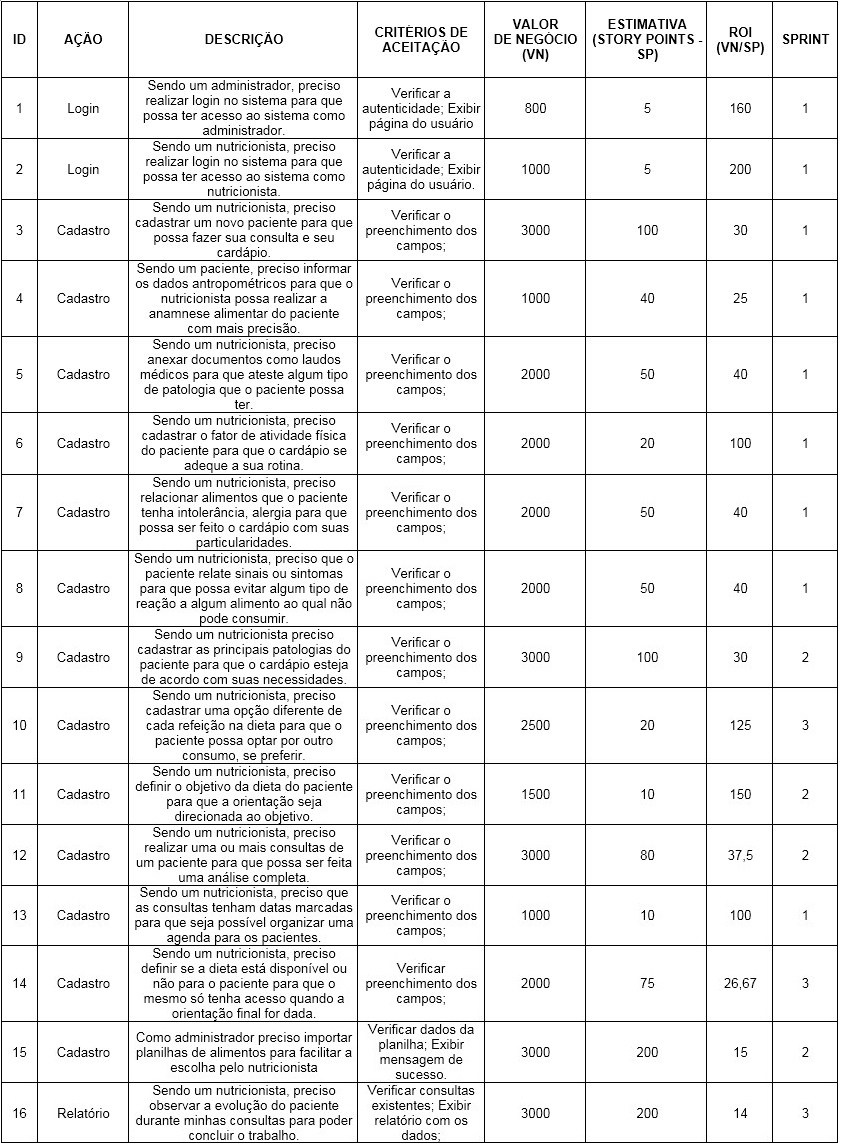
\includegraphics[width=0.90\textwidth]{table.jpg}
\end{center}
\end{figure}

O \textit{Product BackLog} possui oito atributos, especificados na Figura 4:

\begin{enumerate}

\item \textbf{ID}: identifica unicamente uma história do Product BackLog.
\item \textbf{Ação}: define onde deve ser executado a história.
\item \textbf{Descrição}: contém a história de usuário
\item \textbf{Critérios de aceitação}: contém os critérios para que a ação possa ser
executada com êxito.
\item \textbf{Valor de Negócio}: define a importância da história.
\item \textbf{Estimativa (\textit{Story Points})}: estima o custo do (na visão do desenvolvedor)
para se implementar a história.
\item \textbf{ROI (VN/SP)}: retorno do investimento em relação ao custo.
\item \textbf{\textit{Sprint}}: define em que \textit{Sprint} a funcionalidade foi implementada.

\end{enumerate}

\section{Casos de Uso}

Com base nas histórias elencadas no \textit{Product BackLog}, o sistema foi divido em 2
subsistemas. O primeiro define as ações do administrador e do nutricionista. A Figura 5
mostra o diagrama de casos de uso.

\begin{figure} [hbt] 
\label{table1} 
\caption{Casos de Uso Administrador e Nutricionista}
\begin{center}
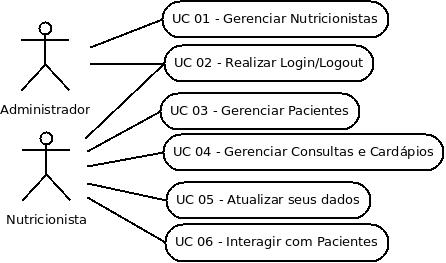
\includegraphics[width=0.75\textwidth]{uc1.jpeg}
\end{center}
\end{figure}

\begin{itemize}
\item \textbf{UC01 – Gerencia Nutricionistas}

\textbf{- Ator:} Administrador

\textbf{- Descrição:} O usuário administrador pode cadastrar, excluir e
editar os nutricionistas do sistema.

\item \textbf{UC02 – Realiza login e logout}

\textbf{- Ator:} Administrador e Nutricionista

\textbf{- Descrição:} Todos os usuários devem se autenticar, para que o
sistema os identifique e defina suas permissões de acesso.

\item \textbf{UC03 – Gerencia Pacientes}

\textbf{- Ator:} Nutricionista

\textbf{- Descrição:} O nutricionista pode cadastrar, editar e excluir
pacientes do sistema.

\item \textbf{UC04 – Gerencia Consultas/Cardápios}

\textbf{- Ator:} Nutricionista

\textbf{- Descrição:} O nutricionista pode cadastrar, editar e excluir
consultas e cardápios feitas sobre um paciente.

\item \textbf{UC05 – Atualiza seus dados}

\textbf{- Ator:} Nutricionista

\textbf{- Descrição:} O nutricionista pode editar dados a seu respeito,
como Nome, E-mail, Senha de Login, etc.

\end{itemize}

O segundo subsistema, deixa claro as ações do nutricionista em relação ao
paciente. A Figura 6 mostra o diagrama de casos de uso desse subsistema.

\begin{figure} [hbt] 
\label{table1} 
\caption{Casos de Uso Nutricionista e Paciente}
\begin{center}
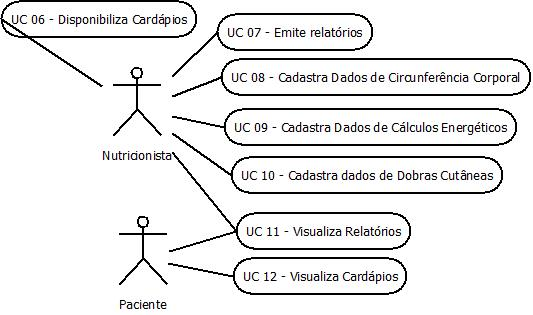
\includegraphics[width=0.75\textwidth]{uc2.jpeg}
\end{center}
\end{figure}

O diagrama da Figura 6 visa deixar claro as principais ações do nutricionista
em relação ao paciente e o que o paciente pode fazer. Abaixo, segue a descrição
detalhada de cada caso de uso:

\begin{itemize}
\item \textbf{UC06 – Disponibiliza cardápios}

\textbf{- Ator:} Nutricionista

\textbf{- Descrição:} Uma vez cadastrado, o nutricionista define se o
cardápio está ou não disponível para o paciente.

\item \textbf{UC07 – Emite relatórios}

\textbf{- Ator:} Nutricionista

\textbf{- Descrição:} O nutricionista é capaz de emitir e disponibilizar
relatórios ao paciente.

\item \textbf{UC08 – Cadastrar Dados de Circunferência Corporal}

\textbf{- Ator:} Nutricionista

\textbf{- Descrição:} O nutricionista deve cadastrar dados de
circunferência corporal, como circunferência da cintura, abdômen,
etc.

\item \textbf{UC09 – Cadastrar Dados de Cálculos Energéticos}

\textbf{- Ator:} Nutricionista

\textbf{- Descrição:} O nutricionista deve cadastrar dados de cálculos
energéticos, como peso, altura, massa livre, etc.

\item \textbf{UC10 – Cadastrar dados de Dobras Cutâneas}

\textbf{- Ator:} Nutricionista

\textbf{- Descrição:} O nutricionista deve cadastrar dados de dobras
cutâneas, como dobra tricipital, abdominal, etc.

\item \textbf{UC11 – Visualiza Relatórios}

\textbf{- Ator:} Paciente

\textbf{- Descrição:} O paciente deve ser capaz de visualizar relatórios
emitidos pelo nutricionista.

\item \textbf{UC12 – Visualiza Cardápios}

\textbf{- Ator:} Paciente

\textbf{- Descrição:} O paciente deve ser capaz de visualizar relatórios
emitidos pelo nutricionista.

\end{itemize}

A Figura 7, relaciona os principais atores do sistema e seus respectivos dados.

\begin{figure} [hbt] 
\label{diagClass1} 
\caption{Diagrama de Classes do Sistema}
\begin{center}
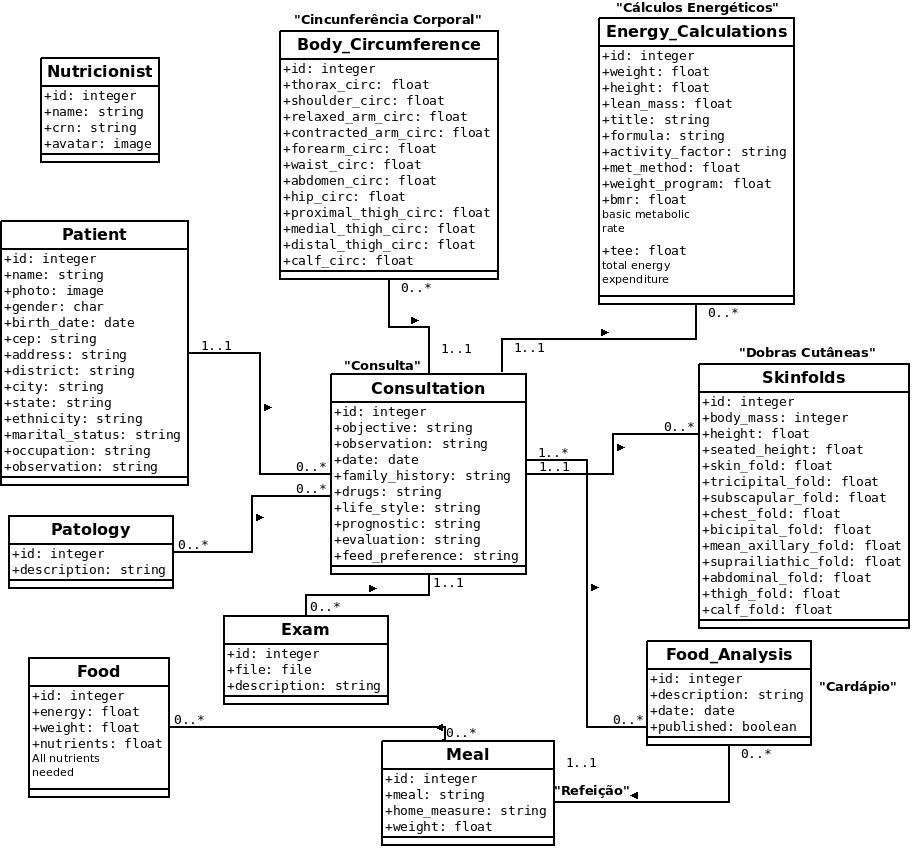
\includegraphics[width=0.75\textwidth]{bd-sistema.jpeg}
\end{center}
\end{figure}

O nutricionista é quem cadastra novos pacientes. O paciente possui dados como
dobras cutâneas, circunferência corporal e dados para cálculos energéticos. O
paciente também pode possuir patologias, onde estas podem interferir na sua
alimentação. Além disso, poderá ser cadastrado exames feitos sobre um paciente. 

Dados como etnia, profissão podem influenciar no fator de atividade física e portanto,
enfatiza-se a presença destes no diagrama da Figura 7.

Cada alimento, possui micro e macro nutrientes como energia, carboidratos,
lipídios, etc. Estes devem ser previamente cadastrados antes de prescrever o
cardápio.

Durante o cadastro de um novo cardápio, o nutricionista seleciona o alimento,
o horário em que será consumido, a quantidade normal, a medida caseira e se este
será publicado ou não, podendo ser editado posteriormente.

\section{Telas do sistema}

Nesta seção, são apresentadas telas, obtidas durante a implementação do sistema.

\begin{figure} [hbt] 
\label{menuNut} 
\caption{Menu do Nutricionista}
\begin{center}
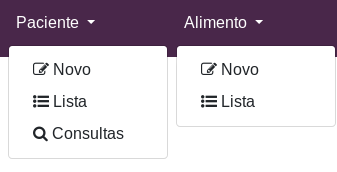
\includegraphics[width=0.55\textwidth]{menuNut1.png}
\end{center}
\end{figure}

\begin{figure} [hbt] 
\label{menuPac} 
\caption{Menu do Paciente}
\begin{center}

\includegraphics[width=0.55\textwidth]{menuPac1.png}
\end{center}
\end{figure}

É possível observar que ambos (paciente e nutricionista) podem ter acesso as suas funcionalidades que ficam localizadas
na barra superior do navegador.

A Figura 8 mostra todas as funcionalidades do Nutricionista. O Nutricionista
ainda pode emitir relatórios a partir da lista de pacientes acessível no menu. Cada
funcionalidade dessa fica disponível a partir do momento que o Nutricionista realiza 
Login no sistema. A Figura 9 mostra o menu do Paciente. O paciente pode obter dados
do relatório ou do cardápio apenas digitando seu ID e senha do sistema.

Como já mencionado anteriormente, o \textit{Django} possui um sistema de URL's e é através dele que
é feito o tratamento de permissões, uma vez que somente o nutricionista é autorizado de fazer cadastro
de pacientes. A Figura 10 mostra um exemplo de lista de usuários previamente cadastrados no sistema.

\begin{figure} [hbt]
\label{listUser} 
\caption{Lista de Usuários Cadastrados}
\begin{center}
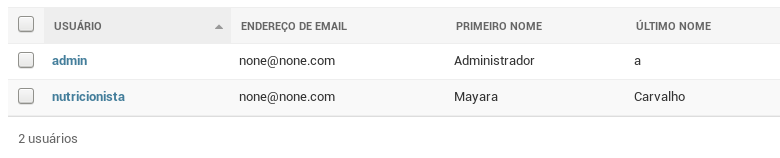
\includegraphics[width=0.55\textwidth]{listaUsuarios.png}
\end{center}
\end{figure}

A Figura 11 mostra a tela de cadastro de pacientes, onde é possível cadastrar
seus dados pessoais e os demais dados para fins de acompanhamento do paciente. 

\begin{figure} [hbt]
\label{cadastroPac} 
\caption{Tela de Cadastro de Pacientes}
\begin{center}
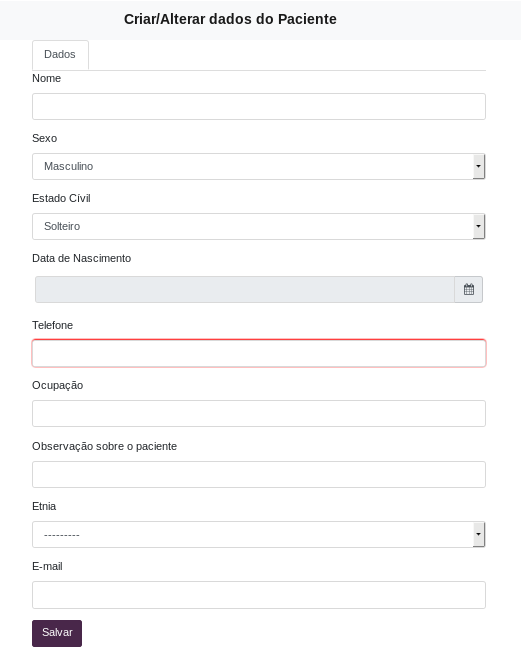
\includegraphics[width=0.55\textwidth]{cadastroPac1.png}
\end{center}
\end{figure}

\begin{figure} [hbt]
\label{cadastroCard} 
\caption{Tela de Cadastro de Cardápio}
\begin{center}
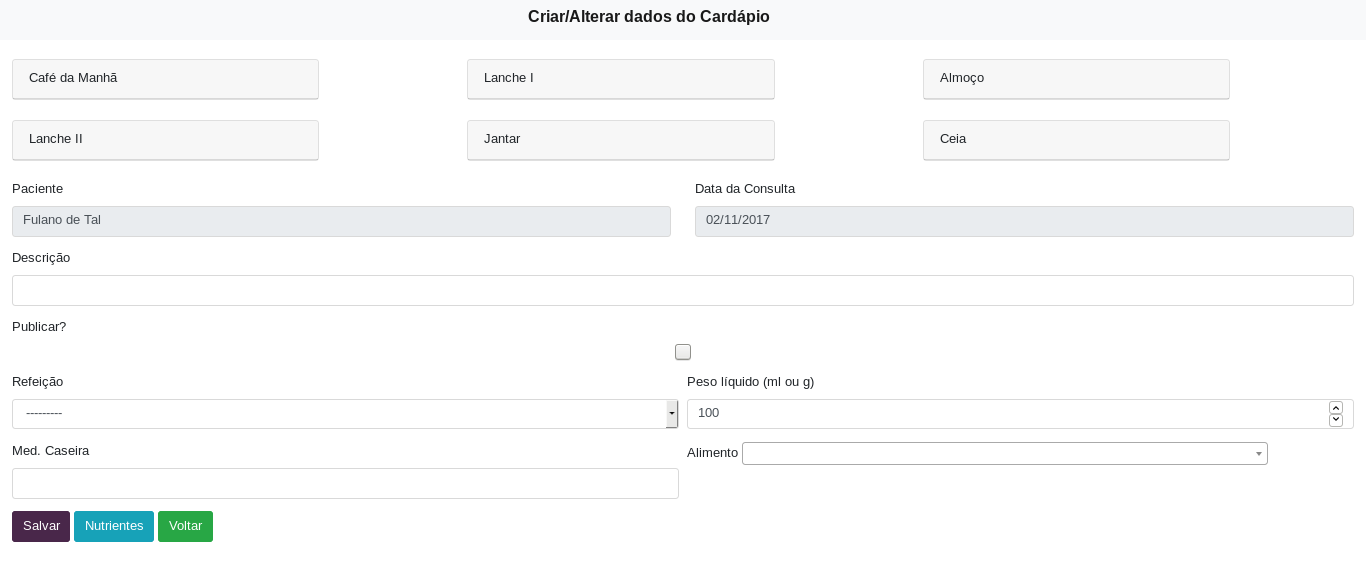
\includegraphics[width=0.55\textwidth]{cadastroCard.png}
\end{center}
\end{figure}

\begin{figure} [hbt]
\label{cadastroCons} 
\caption{Tela de Cadastro de Consulta}
\begin{center}
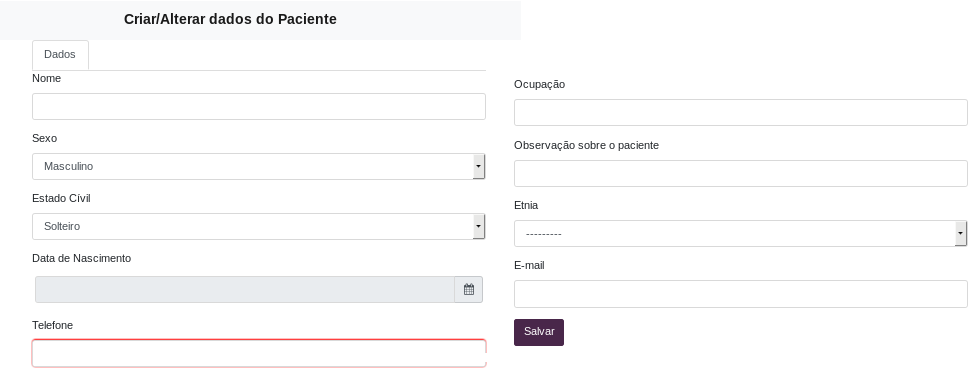
\includegraphics[width=0.55\textwidth]{cadastroCons1.png}
\end{center}
\end{figure}

As Figuras 12 e 13 mostram as telas de cadastro de cardápio e consulta,
respectivamente. É durante a consulta que o nutricionista cadastra os dados de
acompanhamento do paciente. O cardápio só poderá ser cadastrado se a consulta já
tiver sido cadastrada previamente.

No cadastro de consultas, o nutricionista cadastra informações de histórico
familiar do paciente, patologias, fármacos que utiliza, além de dados de
acompanhamento como dobras cutâneas, circunferência corporal, entre outros.

O cadastro de cardápio consta dados do paciente, como nome completo e data
em que a consulta foi realizada. Em seguida, a descrição do cardápio, disponibilidade
e os alimentos a serem cadastrados, que devem ter horário de consumo, quantidade
e medida caseira.

\begin{figure} [hbt]
\label{relatPac} 
\caption{Relatório do Paciente}
\begin{center}
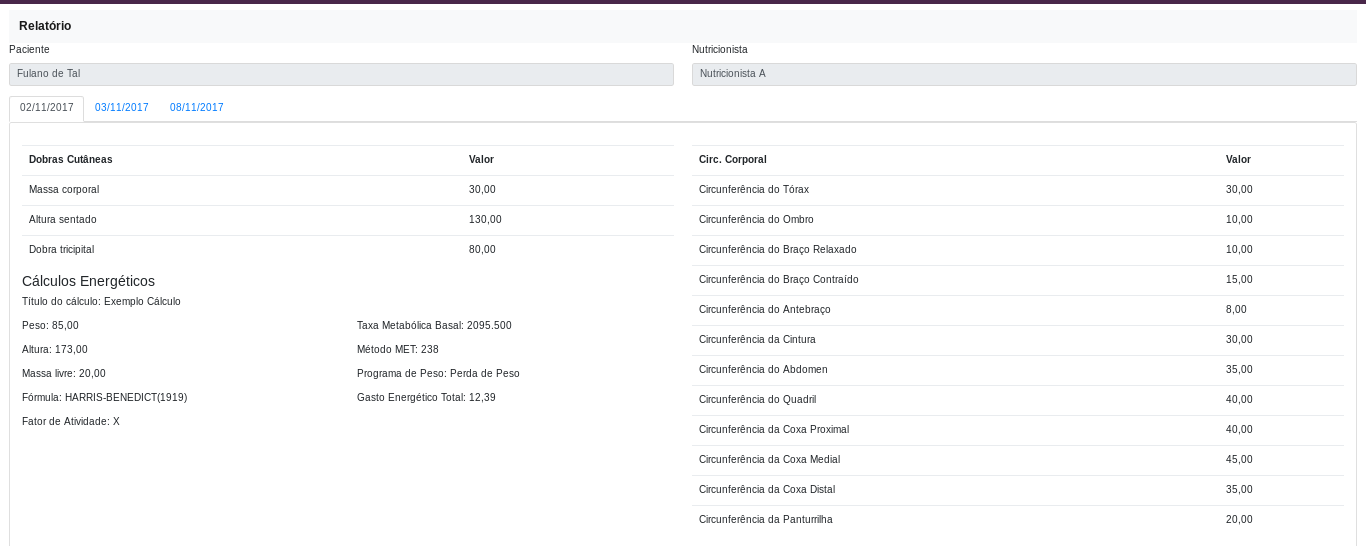
\includegraphics[width=0.75\textwidth]{relatPac1.png}
\end{center}
\end{figure}

A Figura 14 mostra o relatório do paciente, onde é possível ver todos os dados
durante as consultas que foram realizadas e os dados de acompanhamento que foram
obtidos em cada uma delas.

A Figura 15 mostra o cardápio com a descrição e todas as suas informações
nutricionais (macro e micro nutrientes), além do nome do paciente para quem foi
prescrito.
Todas as funcionalidades aqui apresentadas, atualmente, encontram-se
implementadas, onde agora são realizados testes com nutricionistas e pacientes, o público-alvo.

\begin{figure} [hbt]
\label{cardPac} 
\caption{Cardápio do Paciente}
\begin{center}
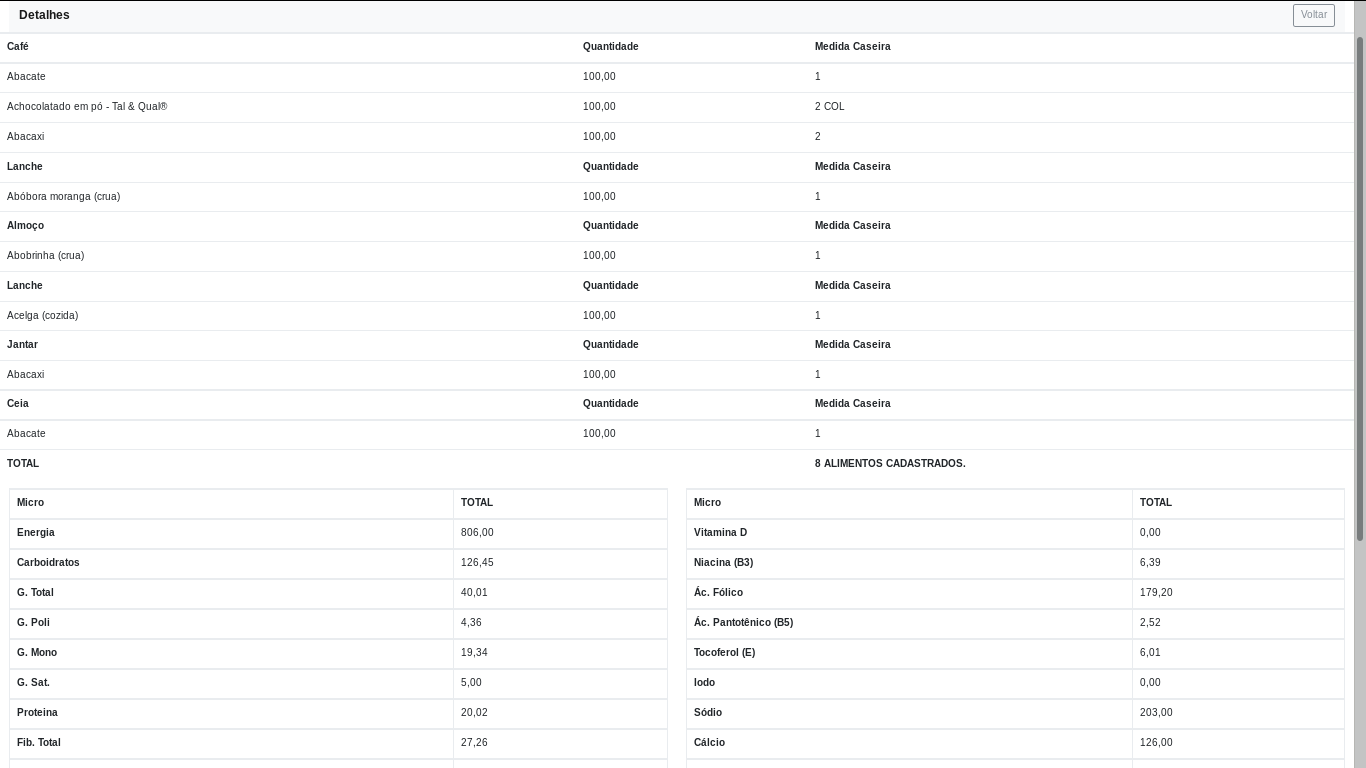
\includegraphics[width=1.0\textwidth]{cardPac1.png}
\end{center}
\end{figure}

\chapter{Resultados e Discussão}

Com base no levantamento de requisitos, representado pelas histórias de usuário, foi desenvolvido o sistema. Foram realizados testes com três potenciais usuários do sistema, buscando uma avaliação do ponto de vista destas pessoas.

O primeiro usuário observou do ponto de vista de um nutricionista e relatou que o sistema é bem simples e que atenderia suas necessidades primárias durante o atendimento de um paciente. Sugeriu que o sistema dispusesse de um chat para conversar com os pacientes durante o acompanhamento nutricional.

O segundo usuário também observou do ponto de vista de um nutricionista e relatou que o sistema precisava de mais informações técnicas a respeito das patologias, mas que continha as informações essenciais para atender e acompanhar um paciente.

Por fim, o terceiro usuário observou do ponto de vista do paciente. Relatou que as informações do seu cardápio e seu relatório se mostravam claras e objetivas. Também sugeriu que ele pudesse interagir com o nutricionista quando fosse necessário a fim de tirar dúvidas sobre o acompanhamento.

A Figura 16 traz o resumo da opinião dos três usuários e a classificação dos mesmos diante a opinião relatada. A classificação pode ser dada em 3 níveis: bom, regular e ruim.

\begin{figure} [hbt]
\label{cardPac} 
\caption{Cardápio do Paciente}
\begin{center}
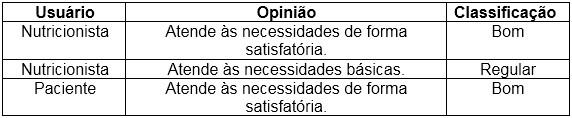
\includegraphics[width=1.0\textwidth]{table4.jpg}
\end{center}
\end{figure}

Todos os usuários que opinaram sobre o sistema são membros do corpo discente da Universidade Federal do Piauí, Campus Senador Helvídio Nunes de Barros.

% ---
% Conclusão
% ---
\chapter{Conclusão}

O presente trabalho trata de um sistema para nutricionista com o intuito de ajudar a fazer o acompanhamento de dietas com seus pacientes de forma gratuita para ambos, tanto paciente como nutricionista. Foi desenvolvido uma ferramenta simples e que atende as
principais necessidades relatadas pelos usuários.

Para solucionar tais problemas, desenvolveu-se um sistema \textit{web} com as
principais funcionalidades elencadas nas histórias de usuário, possibilitando assim
que qualquer usuário (nutricionista ou paciente) pudesse acessá-lo de qualquer
dispositivo com acesso à internet.

Antes de começar o desenvolvimento, estudou-se o problema e entendeu-se
quais as principais necessidades: o trabalho repetitivo e cansativo de calcular as
informações nutricionais de um cardápio, a falta de uma agenda que interaja com os
dados de acompanhamento nutricional. Com base nisso, foi realizado o levantamento de
requisitos através das histórias de usuário para só então passar para a fase de
desenvolvimento.

Como trabalhos futuros, planeja-se ampliar o sistema de modo que o paciente
possa interagir mais com o nutricionista e posteriormente, disponibilizar um aplicativo
móvel, para que o paciente possa receber notificações enviadas pelo seu próprio
nutricionista, facilitando e melhorando o acompanhamento do mesmo.

% ----------------------------------------------------------
% ELEMENTOS PÓS-TEXTUAIS
% ----------------------------------------------------------
\postextual


% ----------------------------------------------------------
% Referências bibliográficas
% ----------------------------------------------------------
\bibliography{references} %% REFERENCIA AO ARQUIVO abntex2-modelo-references.bib

% ----------------------------------------------------------
% Glossário
% ----------------------------------------------------------
%
% Consulte o manual da classe abntex2 para orientações sobre o glossário.
%
%\glossary

% ----------------------------------------------------------
% Apêndices
% ----------------------------------------------------------

% ---
% Inicia os apêndices
% ---
%%\begin{apendicesenv}

% Imprime uma página indicando o início dos apêndices
%%\partapendices

% ----------------------------------------------------------
%%\chapter{Apêndice}
% ----------------------------------------------------------


%%\end{apendicesenv}
% ---



\end{document}
